\section{Results}
    \subsection{Verification of relationship between $r$ and $s$}
        Here we will verify that
        \begin{equation}
            s = 1 + \num{2.5} + \log r.
        \end{equation}

    \begin{figure}[h]
        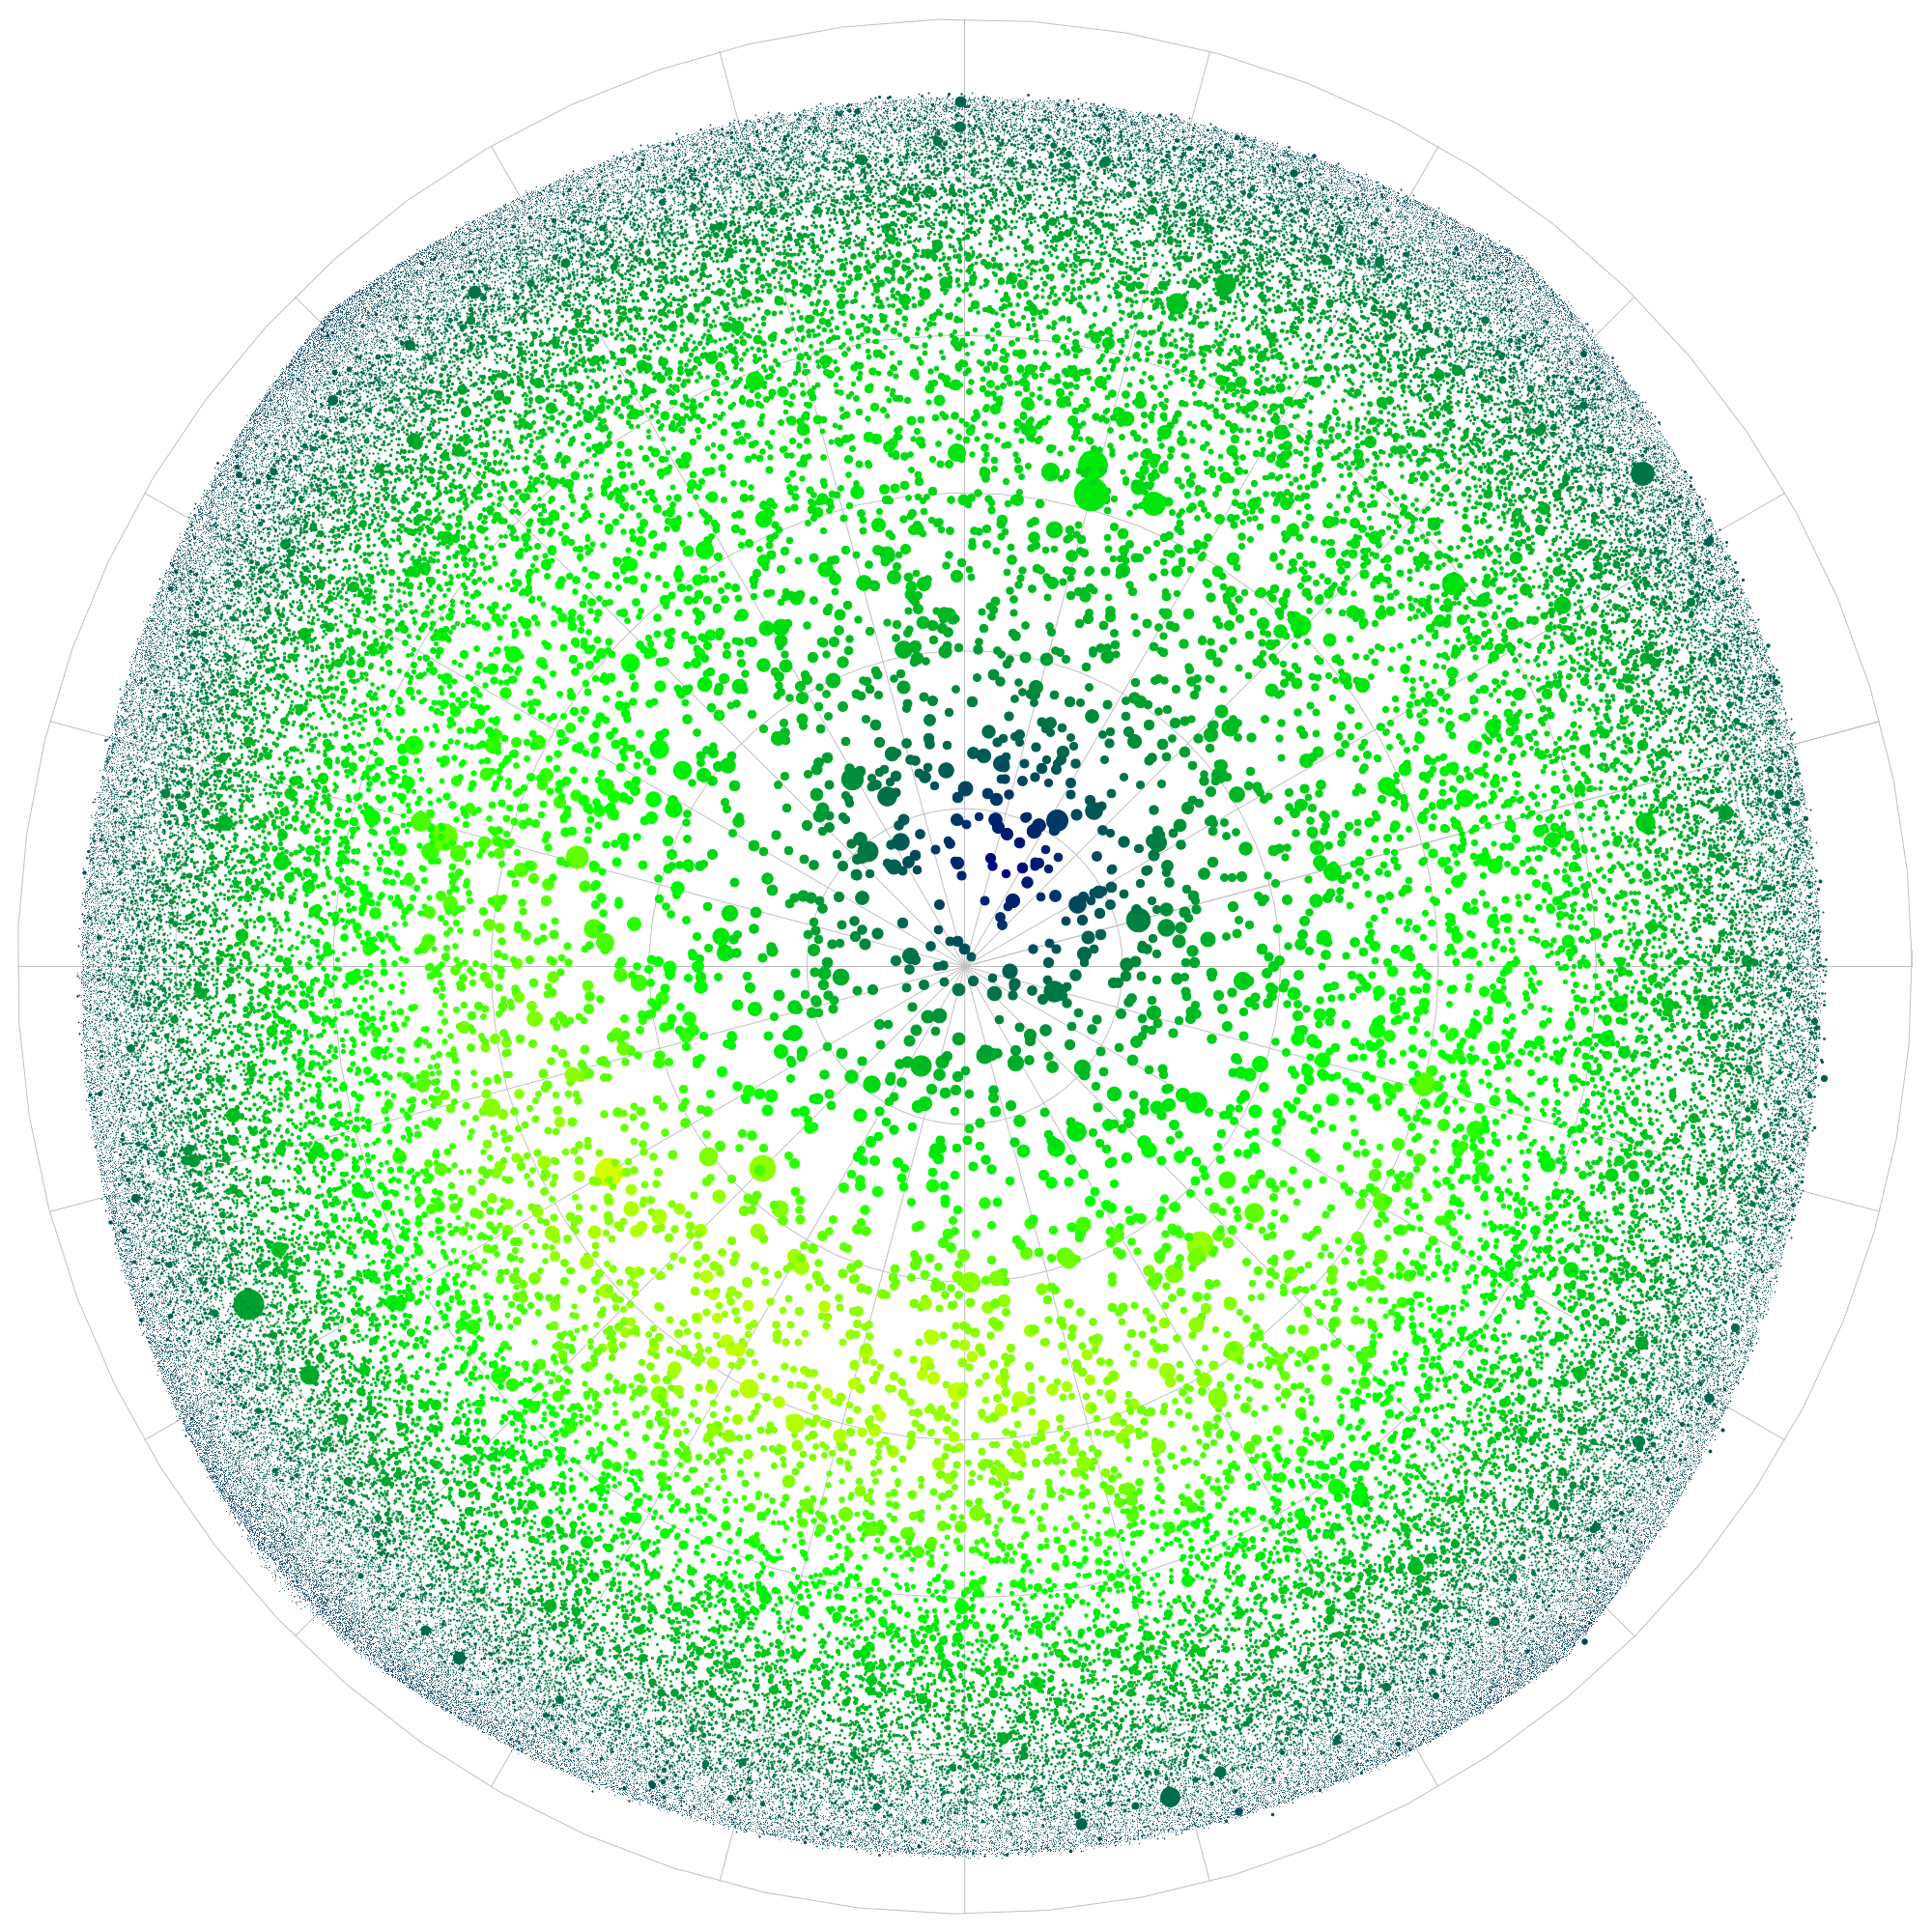
\includegraphics[width = \linewidth]{pictures/angularSpeed-ago.png}
        \caption{A set of 131072 meteors as observed from AGO Modra. Only the brightest frame is displayed for every meteor.
            Size of the dots represents the maximum brightness. Brighter colours correspond to higher observed angular speeds:
            meteors close to the horizon are at large distances, while velocities of meteors observed near the radiant have
            small radial components. Angular speeds are generally highest \ang{90} from the radiant.}
        \label{sim:res:as:as-ago}
    \end{figure}
    
    \begin{figure}
        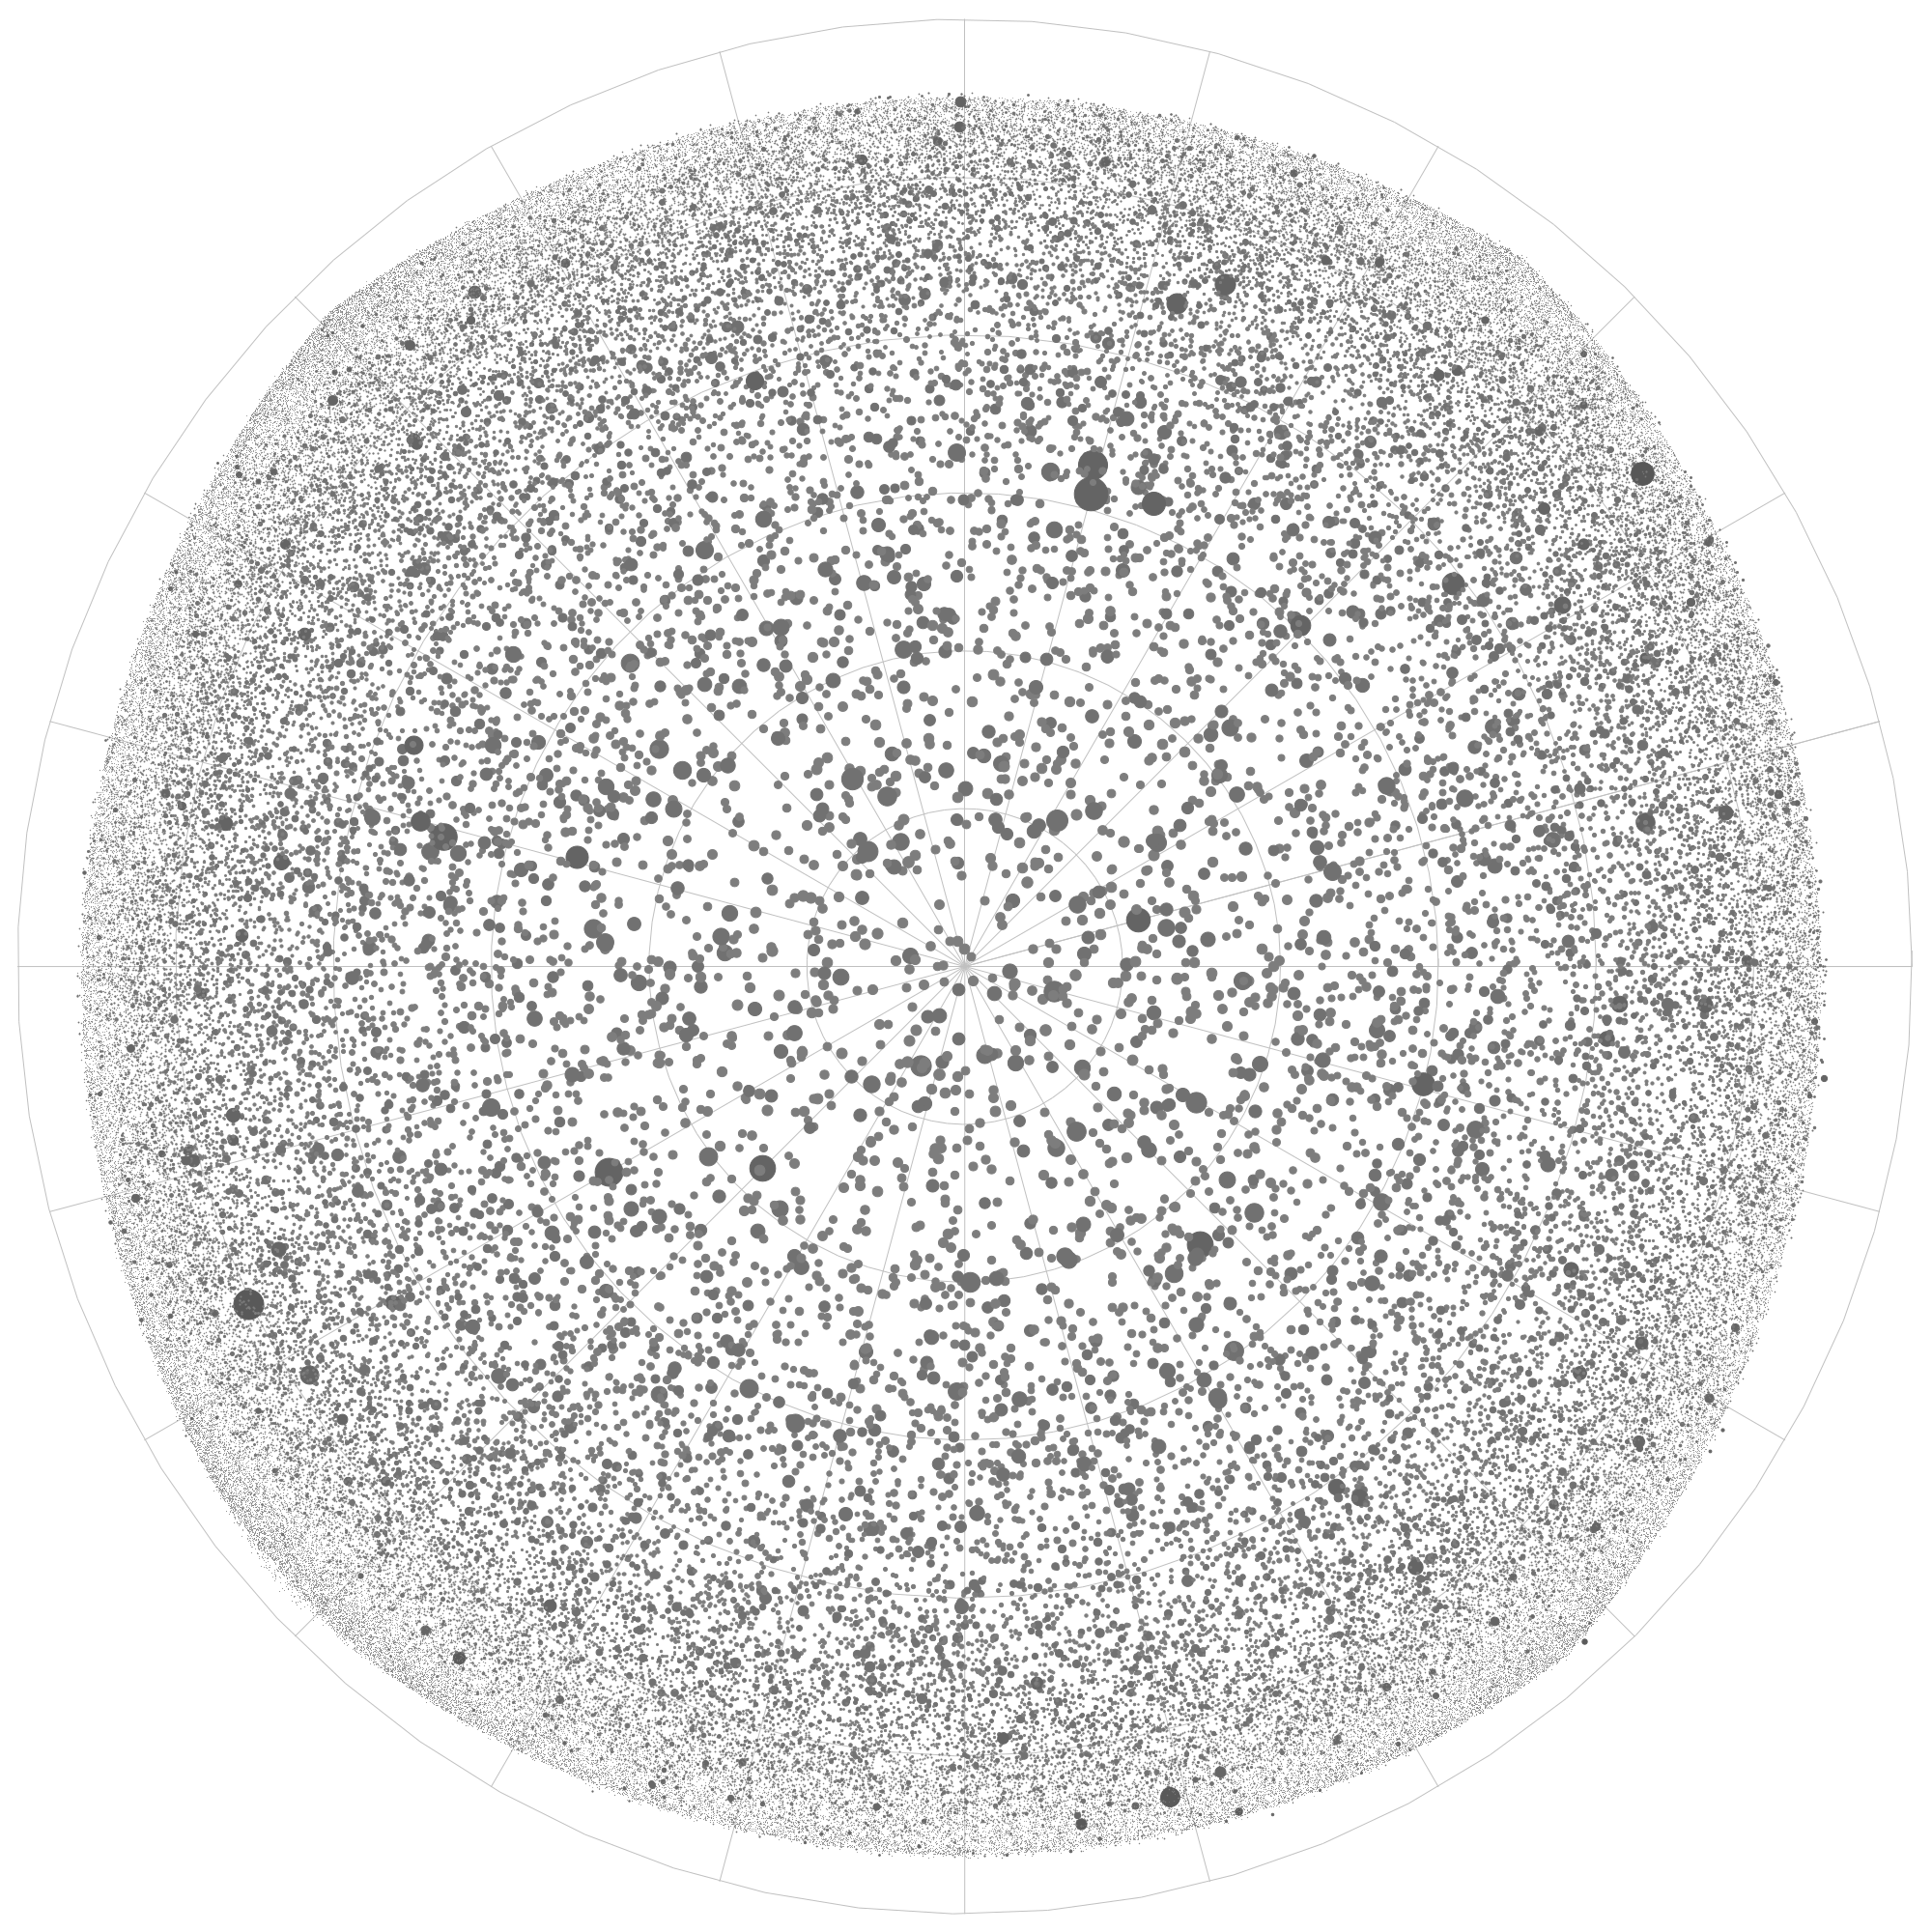
\includegraphics[width = \linewidth]{pictures/elevation-ago.png}
        \caption{The same dataset, coloured by elevation of the meteoroid at the time of maximum brightness. Darker dots represent lower elevations
            and thus generally correspond to larger particles at greater penetration depths.}
        \label{sim:res:as:ele-ago}
    \end{figure}
